\documentclass[a4paper,11pt]{book}
\usepackage{listings}
\usepackage[utf8]{inputenc}
\usepackage[spanish, es-tabla]{babel}

\usepackage{titlesec}
\usepackage{fancyhdr}
\usepackage[hidelinks]{hyperref}
\usepackage{xcolor}
\usepackage{pdfpages}

\usepackage{xspace}

\usepackage{datatool}% http://ctan.org/pkg/datatool

% ********************************************************************
% Información reutilizable
% ********************************************************************
\newcommand{\mySubject}{Trabajo Fin de Grado\xspace}
\newcommand{\myTitle}{Hearcloud\xspace}
\newcommand{\mySubTitle}{Aplicación web orientada a la organización y gestión de música online\xspace}
\newcommand{\mySubTitleENG}{Web application for music management\xspace}
\newcommand{\myDegree}{Grado en Ingeniería Informática\xspace}
\newcommand{\myName}{Mariano Palomo Villafranca\xspace}
\newcommand{\myEmail}{mpvillafranca@correo.ugr.es\xspace}
\newcommand{\myDNI}{20100242J\xspace}
\newcommand{\myProf}{José María Guirao Miras\xspace}
\newcommand{\myFaculty}{Escuela Técnica Superior de Ingenierías Informática y de
Telecomunicación\xspace}
\newcommand{\myFacultyShort}{E.T.S. de Ingenierías Informática y de
Telecomunicación\xspace}
\newcommand{\myDepartment}{Departamento de Lenguajes y Sistemas Informáticos\xspace}
\newcommand{\myUni}{\protect{Universidad de Granada}\xspace}
\newcommand{\myLocation}{Granada\xspace}
\newcommand{\myTime}{\today\xspace}
\newcommand{\myVersion}{Version 0.1\xspace}

% ********************************************************************
% Información de archivo
% ********************************************************************
\hypersetup{
pdfauthor = {\myName (\myEmail)},
pdftitle = {\myTitle},
pdfsubject = {\mySubject},
pdfkeywords = {Hearcloud, aplicación web, música, Django, software libre},
pdfcreator = {LaTeX con el paquete Texmaker},
pdfproducer = {pdflatex}
}

% ********************************************************************
% Estilo de cabeceras
% ********************************************************************
\pagestyle{fancy}
\fancyhf{}
\fancyhead[LO]{\leftmark}
\fancyhead[RE]{\rightmark}
\fancyhead[RO,LE]{\textbf{\thepage}}
\setlength{\headheight}{1.5\headheight}

% ********************************************************************
% Redefinición de comandos
% ********************************************************************
\renewcommand{\chaptermark}[1]{\markboth{\textbf{#1}}{}}
\renewcommand{\sectionmark}[1]{\markright{\textbf{\thesection. #1}}}

% ********************************************************************
% Definición de colores
% ********************************************************************
\definecolor{gray97}{gray}{.97}
\definecolor{gray75}{gray}{.75}
\definecolor{gray45}{gray}{.45}
\definecolor{gray30}{gray}{.94}

% ********************************************************************
% Listados
% ********************************************************************
\lstset{ frame=Ltb,
     framerule=0.5pt,
     aboveskip=0.5cm,
     framextopmargin=3pt,
     framexbottommargin=3pt,
     framexleftmargin=0.1cm,
     framesep=0pt,
     rulesep=.4pt,
     backgroundcolor=\color{gray97},
     rulesepcolor=\color{black},
     %
     stringstyle=\ttfamily,
     showstringspaces = false,
     basicstyle=\scriptsize\ttfamily,
     commentstyle=\color{gray45},
     keywordstyle=\bfseries,
     %
     numbers=left,
     numbersep=6pt,
     numberstyle=\tiny,
     numberfirstline = false,
     breaklines=true,
   }
 
% Minimizar fragmentado de listados
\lstnewenvironment{listing}[1][]
   {\lstset{#1}\pagebreak[0]}{\pagebreak[0]}

% ********************************************************************
% Estilo de listados de código
% ********************************************************************
\lstdefinestyle{CodigoC}
   {
	basicstyle=\scriptsize,
	frame=single,
	language=C,
	numbers=left
   }
\lstdefinestyle{CodigoC++}
   {
	basicstyle=\small,
	frame=single,
	backgroundcolor=\color{gray30},
	language=C++,
	numbers=left
   }

 
\lstdefinestyle{Consola}
   {basicstyle=\scriptsize\bf\ttfamily,
    backgroundcolor=\color{gray30},
    frame=single,
    numbers=none
   }


\newcommand{\bigrule}{\titlerule[0.5mm]}


% ********************************************************************
% Para ordenar listas de elementos
% ********************************************************************
\newcommand{\sortitem}[1]{%
  \DTLnewrow{list}% Create a new entry
  \DTLnewdbentry{list}{description}{#1}% Add entry as description
}
\newenvironment{sortedlist}{%
  \DTLifdbexists{list}{\DTLcleardb{list}}{\DTLnewdb{list}}% Create new/discard old list
}{%
  \DTLsort{description}{list}% Sort list
  \begin{itemize}%
    \DTLforeach*{list}{\theDesc=description}{%
      \item \theDesc}% Print each item
  \end{itemize}%
}

% ********************************************************************
% Para que en las páginas en blanco no tengan cabeceras
% ********************************************************************
\makeatletter
\def\clearpage{%
  \ifvmode
    \ifnum \@dbltopnum =\m@ne
      \ifdim \pagetotal <\topskip
        \hbox{}
      \fi
    \fi
  \fi
  \newpage
  \thispagestyle{empty}
  \write\m@ne{}
  \vbox{}
  \penalty -\@Mi
}
\makeatother

% ********************************************************************
% Memoria
% ********************************************************************
\begin{document}
\begin{titlepage}
 
\newlength{\centeroffset}
\setlength{\centeroffset}{-0.5\oddsidemargin}
\addtolength{\centeroffset}{0.5\evensidemargin}

\noindent\hspace*{\centeroffset}\begin{minipage}{\textwidth}

\centering

\includegraphics[width=0.9\textwidth]{../images/logo_ugr.jpg}\\[1.4cm]

\textsc{\Large\mySubject\\[0.2cm]}
\textsc{\myDegree}\\[1cm]

{\Huge\bfseries \myTitle\\}
\noindent\rule[-1ex]{\textwidth}{3pt}\\[3.5ex]
{\large\bfseries \mySubtitle}
\end{minipage}

\vspace{2.5cm}
\noindent\hspace*{\centeroffset}\begin{minipage}{\textwidth}
\centering

\textbf{Autor}\\ {\myName}\\[2.5ex]
\textbf{Tutor}\\ {Prof. Dr. \myProf}\\[2cm]

\includegraphics[width=0.3\textwidth]{../images/etsiit_logo.png}\\[0.1cm]
\textsc{\myFaculty}\\
\textsc{---}\\
\myLocation, \myTime\\

\includegraphics[width=0.3\textwidth]{../images/CC-SA-logo.png}
\end{minipage}
\end{titlepage}



\begin{titlepage}
 
 
\setlength{\centeroffset}{-0.5\oddsidemargin}
\addtolength{\centeroffset}{0.5\evensidemargin}
\thispagestyle{empty}

\noindent\hspace*{\centeroffset}\begin{minipage}{\textwidth}

\centering

\vspace{3.3cm}

% Logo del proyecto

\includegraphics[width=0.5\textwidth]{../images/logo_hearcloud_full.png}

 \vspace{0.5cm}

% Title

{\Huge\bfseries \myTitle\\
}
\noindent\rule[-1ex]{\textwidth}{3pt}\\[3.5ex]
{\large\bfseries \mySubTitle.\\[4cm]}
\end{minipage}

\vspace{2.5cm}
\noindent\hspace*{\centeroffset}\begin{minipage}{\textwidth}
\centering

\textbf{Autor}\\ {\myName}\\[2.5ex]
\textbf{Tutor}\\ {Prof. Dr. \myProf}\\[2cm]

\end{minipage}
\vspace{\stretch{2}}

 
\end{titlepage}




\begin{center}
{\large\bfseries \myTitle. \mySubTitle}\\
\end{center}
\begin{center}
\myName\\
\end{center}

% ********************************************************************
% Resumen (Español)
% ********************************************************************
\section*{Resumen}

\bigskip
\noindent{\textbf{Palabras clave}: \textit{aplicación web}, \textit{cloud}, \textit{música}, \textit{organización}, \textit{servidor}, \textit{cliente} }\\

Se pretende desarrollar una \textit{aplicación web} que permita el almacenamiento de ficheros de \textit{música} teniéndolos disponibles en cualquier momento y lugar que se desee, facilitando su accesibilidad a modo de plataforma de computación en la nube (\textit{cloud}). Como resultado, tendremos una herramienta útil y sencilla orientada a la organización de la biblioteca musical del usuario, que podrá realizar modificaciones sobre los metadatos de sus ficheros, tales como ``título'', ``artista'' o ``portada'' y descargarlos de nuevo al sistema local, si quiere, tras los cambios realizados.

El proyecto estará basado en su totalidad en el \textit{software libre}, pudiendo ser adaptado sin dificultad por cualquier otro usuario que así lo quisiera. El desarrollo del servidor se realizará con {\tt Django}, que es un framework para aplicaciones web gratuito y open source, escrito en {\tt Python} que ayuda a desarrollar sitios web más fácil y rápidamente. Haremos uso de {\tt Django template language (DTL)}, que está inspirado en {\tt Jinja2}, para generar archivos HTML basados en \textit{templates}. Por otra parte, en el lado del cliente, utilizaremos código \textit{CSS} para definir y crear la presentación de los documentos HTML con el framework {\tt Twitter Bootstrap} que contiene plantillas de diseño para tipografía, formularios, botones, cuadros, menús de navegación y otros elementos de diseño y nos simplificará la tarea. También se incluirá código \textit{Javascript} y \textit{jQuery} que ayudará a mejorar la experiencia de usuario durante su navegación por el sistema.

Al tratarse de \textit{software libre}, el desarrollo no está limitado al equipo que inicia el trabajo y cualquier usuario puede hacer una contribución al mismo. Para ello, se utilizará un \textit{sistema de control de versiones}, en este caso, {\tt Git}, que es prácticamente un estándar en el mundo. Además, se empleará la plataforma de desarrollo colaborativo (forja) {\tt Github}, que está integrada con Git y nos ayudará en el desarrollo y la distribución del trabajo. De esta forma, cualquier persona que quiera acceder al código del proyecto, podrá hacerlo a través del repositorio y obtener su propia copia gratuita.


\newpage

% ********************************************************************
% Resumen (Inglés)
% ********************************************************************
\begin{center}
{\large\bfseries \myTitle. \mySubTitleENG}\\
\end{center}
\begin{center}
\myName\\
\end{center}

\section*{Abstract}

\bigskip
\noindent{\textbf{Keywords}: \textit{web application}, \textit{cloud}, \textit{music}, \textit{organiation}, \textit{server}, \textit{client} }\\

This project aims to develop a \textit{web application} that lets store \textit{music} files, having them available at every moment and place you want to as a \textit{cloud computing platform}. As a result, we'll have a simple and useful tool oriented to ma}nage the users musical library, who'll be able to edit the files metadatas, like ``title'', ``artist'' or ``cover artwork'' and download them back into their local system, if they want, after those changes.

The development will be \textit{open source}, which means that other users could easily contribute or re-adapt the code if wanted. The server part (backend) will be done with {\tt Django}, a high-level {\tt Python} Web framework that encourages rapid development and clean, pragmatic design. We'll be using {\tt Django template languaje (DTL)}, which is actually based on {\tt Jinja2} syntax, to generate HTML files from templates. Besides that, on the client side (frontend), we'll use \textit{CSS} code to create and define the presentation of that HTML files with the {\tt Twitter Bootstrap} framework, which contains design patterns for fonts, forms, buttons, navegation menus and other elements and will help to make the things easier. Also, we'll include \textit{Javascript} and \textit{jQuery} code to improve the user experience during his navigation across the plattform.

As it's \textit{open source}, the development it's not limited to the team who starts the project so anyone could contribute to it. That's why we'll be using a \textit{version control system}, {\tt Git}, which it's almost an standard all over the world right now. In adition, a web-based Git repository hosting service called {\tt Github} will be used to manage the project work. That way, everyone who want to access the code, could visit the repository link and get his own free copy.

\newpage

% ********************************************************************
% Autorización de publicación en la biblioteca del centro
% ********************************************************************
%\chapter*{}
\thispagestyle{empty}
\noindent\rule[-1ex]{\textwidth}{2pt}\\[4.5ex]

Yo, \textbf{\myName}, alumno de la titulación \myDegree{} de la \textbf{\myFaculty}, con DNI \myDNI, autorizo la
ubicación de la siguiente copia de mi Trabajo Fin de Grado en la biblioteca del centro para que pueda ser
consultada por las personas que lo deseen.

\bigskip
Así mismo, dicha copia se publica bajo licencia \textbf{Creative Commons Attribution-ShareAlike 4.0}. Los terminos de la licencia permiten su copia y/o adaptación en cualquier medio o formato, siempre y cuando se reconozca la autoría y se redistribuya con la misma licencia que el original. La presente documentación, en formato {\tt LaTeX}, puede encontrarse en el repositorio de {\tt Github}: \url{https://github.com/mpvillafranca/hearcloud-doc}.

\vspace{6cm}

\noindent Fdo: \myName

\vspace{2cm}

\begin{flushright}
\myLocation a \myTime.
\end{flushright}

\newpage


% ********************************************************************
% Tutor
% ********************************************************************
%\chapter*{}
\thispagestyle{empty}
\noindent\rule[-1ex]{\textwidth}{2pt}\\[4.5ex]

D. \textbf{\myProf}, profesor del \myDepartment de la \myUni.

\vspace{0.5cm}

\textbf{Informan:}

\vspace{0.5cm}

Que el presente trabajo, titulado \textit{\textbf{\myTitle, \mySubTitle}}, ha sido realizado bajo su supervisión por \textbf{\myName}, y autoriza la defensa de dicho trabajo ante el tribunal que corresponda.

\vspace{0.5cm}

Y para que conste, expiden y firman el presente informe en \myLocation a \myTime.

\vspace{1cm}

\textbf{El tutor:}

\vspace{5cm}

\noindent \textbf{\myProf}

\chapter*{Agradecimientos}
\thispagestyle{empty}

       \vspace{1cm}


Poner aquí agradecimientos...



\tableofcontents
\listoffigures
\listoftables

\mainmatter
\setlength{\parskip}{5pt}

\chapter{Introducción}
\label{cap:introduccion}

\section{Antecedentes históricos}

En el ámbito de las prácticas culturales y aficiones personales de cualquier sociedad, está muy asentado el gusto por la música, sea del tipo que sea, hecho por el cual resulta inevitable que, con el tiempo, hayan surgido dispositivos que permitieran registrar dichos sonidos y almacenarlos para su posterior reproducción.

La historia contemporánea del registro del sonido comienza en 1857, con el fonoautógrafo de Leon Scott, aunque en 1877, Thomas Edison crea el primer artefacto capaz de grabar y reproducir sonido, el fonógrafo, que rápidamente fue sustituido por el gamófono, debido a sus diversas ventajas con respecto a su predecesor. Más tarde, en 1940, aparece el disco de vinilo, logrando una mayor duración y calidad de sonido. Durante ese mismo año, se desarrolla el magnetófono de bobina abierta, que aporta grabaciones de larga duración y buena fidelidad, hecho por el cual tuvo un gran éxito tanto en uso hogareño como profesional. El casete compacto surge posteriormente basándose en esos mismos principios, seguido del microcasete, minicasete, VHS, Casete Compacto Digital y mini DV. Ya en 1979, se produce uno de los inventos más revolucionarios, el disco compacto, que supuso el primer formato digital para audio, desplazando al disco de vinilo y casete. No obstante, el invento más revolucionario en este ámbito, el formato MP3, se empieza a gestar en 1986 y, en 1995 Brandenburg lo utiliza por primera vez en su propio ordenador, convirtiéndose hoy en día en el formato más popular de audio.

Cada soporte de los aquí descritos, ha llevado consigo una forma diferente de organizar los contenidos musicales por parte de los usuarios, tendiendo a una reducción y optimización del espacio necesario para albergar dicha biblioteca musical. 

Con la introducción en el mercado de los ordenadores personales y los diferentes formatos de archivos de audio digital, las alternativas disponibles para llevar a cabo esta organización han aumentado de manera exponencial y se han visto potenciadas, posteriormente, por la aparición de internet.

\section{Motivación}

Uno de los principales problemas que surgen del almacenamiento de música en los ordenadores personales en la actualidad es su portabilidad, pues existe un gran abanico de posibilidades en cuanto a dispositivos de reproducción se refiere: reproductores MP3, iPods, teléfonos móviles, tabletas, automóviles, etc. 

No obstante, normalmente, el usuario debe elegir un dispositivo en el que almacenar su biblioteca y, si quisiera portarla a otro, copiarla al mismo mediante algún método de transferencia de ficheros. El principal problema de ello, es mantener la sincronización entre estos dispositivos.

Este proyecto surge como respuesta a esa necesidad de los usuarios de organizar su música y mantenerla ``sincronizada'' en todos sus dispositivos, de manera que esté disponible en lugar que se desee.



\chapter{Objetivos}
\label{cap:objetivos}

El objetivo del proyecto es la creación de una plataforma web donde los usuarios puedan almacenar su biblioteca musical y ésta se encuentre disponible para ellos en cualquier lugar y momento que deseen a través de internet. Se pretende establecer una metodología de trabajo flexible, en la que puedan ir incluyéndose mejoras incrementalmente manteniéndose la integridad del sistema. \\

Si bien, éste es el objetivo final a alcanzar, podemos destacar una serie de objetivos principales a cumplir que darán pié al mismo:

\begin{itemize}
	\item \textbf{OBJ-1.} Estudiar el estado actual del mercado en cuanto a productos y soluciones de este tipo, analizando sus ventajas y desventajas correspondientes.

	\item \textbf{OBJ-2.} Proporcionar una metodología flexible y sencilla, pero a la vez robusta y viable que se pueda aplicar durante el desarrollo íntegro del proyecto. 

	\item \textbf{OBJ-3.} Crear un sistema flexible que pueda ser adaptado con facilidad por otros usuarios que así lo deseen, ya sea como contribución al proyecto original o para su propia implantación de manera externa.

	\item \textbf{OBJ-4.} Dotar al proyecto de la posibilidad de ser alojado en la nube, buscando una alta disponibilidad y calidad en la experiencia de usuario.

	\item \textbf{OBJ-5.} Llevar a cabo un desarrollo abierto tanto del proyecto como de su documentación (véase apéndice \hyperref[sec:licencias]{Licencias}), dando como resultado un producto \textit{open source} basado en tecnología libre.
\end{itemize}

\bigskip

\section{Alcance de los objetivos}

La plataforma resultante podrá ser implantada en cualquier servidor en el que quiera desplegarse siempre que puedan satisfacerse las dependencias necesarias. Por otra parte, al tratarse de un sistema \textit{open source} y, puesto que el software es de dominio público, se podría buscar un posible nicho de mercado en la prestación del servicio en la nube.


\chapter{Análisis}


\chapter{Planificación}

\section{Fases y entregas}

\subsection{Fases}

\subsection{Lista de entregas}

\section{Estructura de descomposición del trabajo}

\section{Lista de actividades}

\section{Recursos humanos}

Se contempla la participación de representantes del público objetivo destinatario del producto con el fin de recabar información relativa a su utilidad, así como posibles deficiencias, beneficios y/o mejoras.

\section{Presupuesto}

La principal ventaja del uso de software libre es que no es necesario adquirir licencias de pago para usar dicho software. Como las herramientas que se van a utilizar y todo el código que se genere será libre, el coste económico y, por tanto, el presupuesto inicial del proyecto será cero.

\bigskip

El único aspecto económico relevante que habrá que considerar en este caso será, entonces, el de los posibles gastos por el uso de un servidor en el que se implate el software.

\section{Temporización}


\chapter{Diseño}
\label{cap:disenio}

\chapter{Implementación}
\label{cap:implementacion}


\chapter{Pruebas}
\label{cap:pruebas}


\chapter{Conclusiones y trabajos futuros}


\chapter{Apéndices}
\label{cap:apendices}

\section{Glosario de términos}
\label{sec:glosario}

\begin{sortedlist}
    \sortitem{\textbf{Frontend}: es la interfaz de la aplicación, es la parte de la aplicación que el usuario utiliza para comunicarse con la misma.}

    \sortitem{\textbf{Backend}: es el motor de una aplicación, se encarga de realizar las funciones en segundo plano que se encargan de que la aplicación funcione.}

    \sortitem{\textbf{Cloud}: }

    \sortitem{\textbf{Metadatos}: }

    \sortitem{\textbf{Software libre}: }

    \sortitem{\textbf{Framework}: }

    \sortitem{\textbf{Template}: }

    \sortitem{\textbf{Forja}: }

    \sortitem{\textbf{Streaming}: }

\end{sortedlist}

\newpage


\section{Licencias}
\label{sec:licencias}

El desarrollo del proyecto se ha llevado a cabo con tecnología \textit{open source}, y el código ha sido liberado bajo licencia \textbf{GNU AFFERO GENERAL PUBLIC LICENSE, Version 3} en el repositorio de Github \url{http://github.com/hearcloud/hearcloud}.

La memoria del proyecto se ha liberado bajo copyright \textbf{Creative Commons}, en concreto, \textbf{CC-BY-SA}.

\section{Preámbulo de la licencia}

\newpage

\section{Manual de usuario}
\label{sec:manual}

\subsection{Página principal}

La página principal es accesible cuando el usuario escribe en el navegador la URL raíz y no ha iniciado sesión en el mismo. En esta página encontramos las siguientes secciones:

\begin{itemize}
	\item \textit{What is Hearcloud?}. Describe en qué consiste la plataforma.
	\item \textit{Features}. Presenta las principales características del sistema.
	\item \textit{Contact the developer}. Links para contactar con el desarrollador de la plataforma.
\end{itemize}

Además, se muestran accesibles al usuario en todo momento links a las páginas de inicio de sesión y registro (\textit{sign in} y \textit{sign up})que se describen en la próxima sección.

\begin{figure}[H] 
\centering 
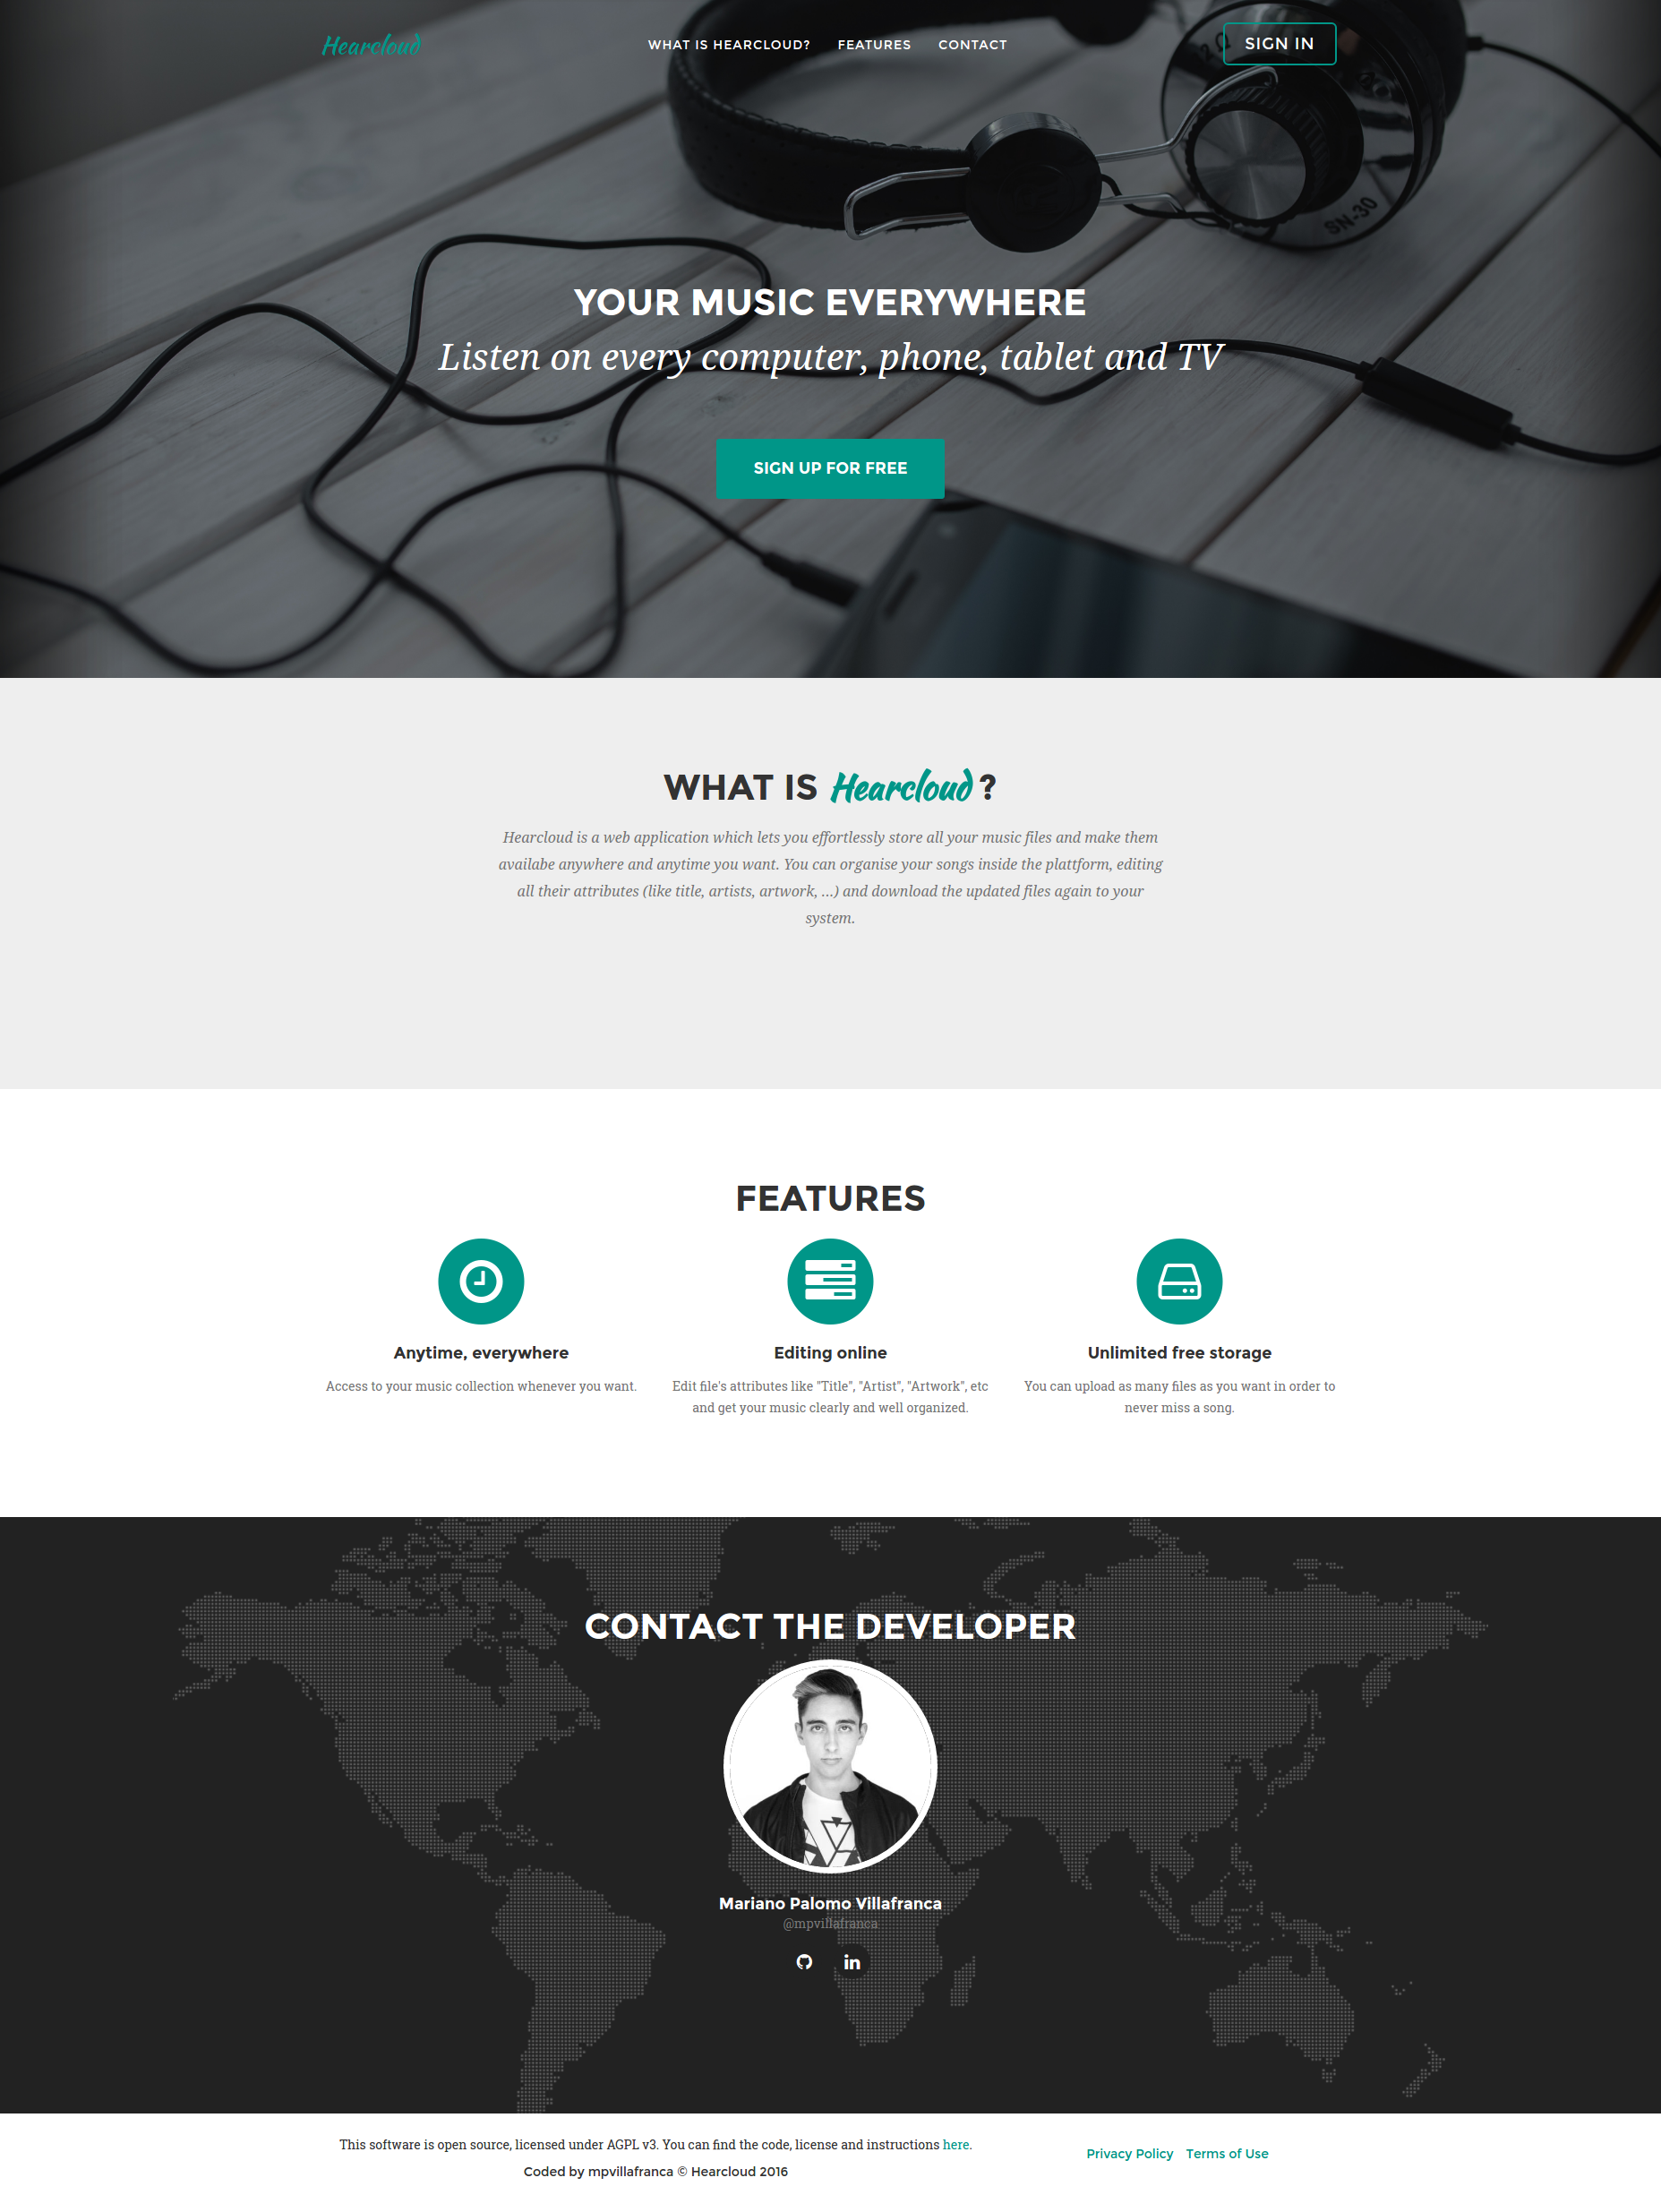
\includegraphics[scale=0.2]{../images/um/um_1.png}
\caption{Página principal (usuario no autenticado)}
\end{figure}

\subsection{Registro y acceso al sistema de usuarios}

La página de registro consiste en un formulario en el que se le solicita al usuario que introduzca un nombre de usuario, un email y una contraseña. Además, se le da la opción de cancelar el registro (lo que le redireccionaría de vuelta a la página principal) o de iniciar sesión (si ya estuviera registrado en el sistema).

\begin{figure}[H] 
\centering 
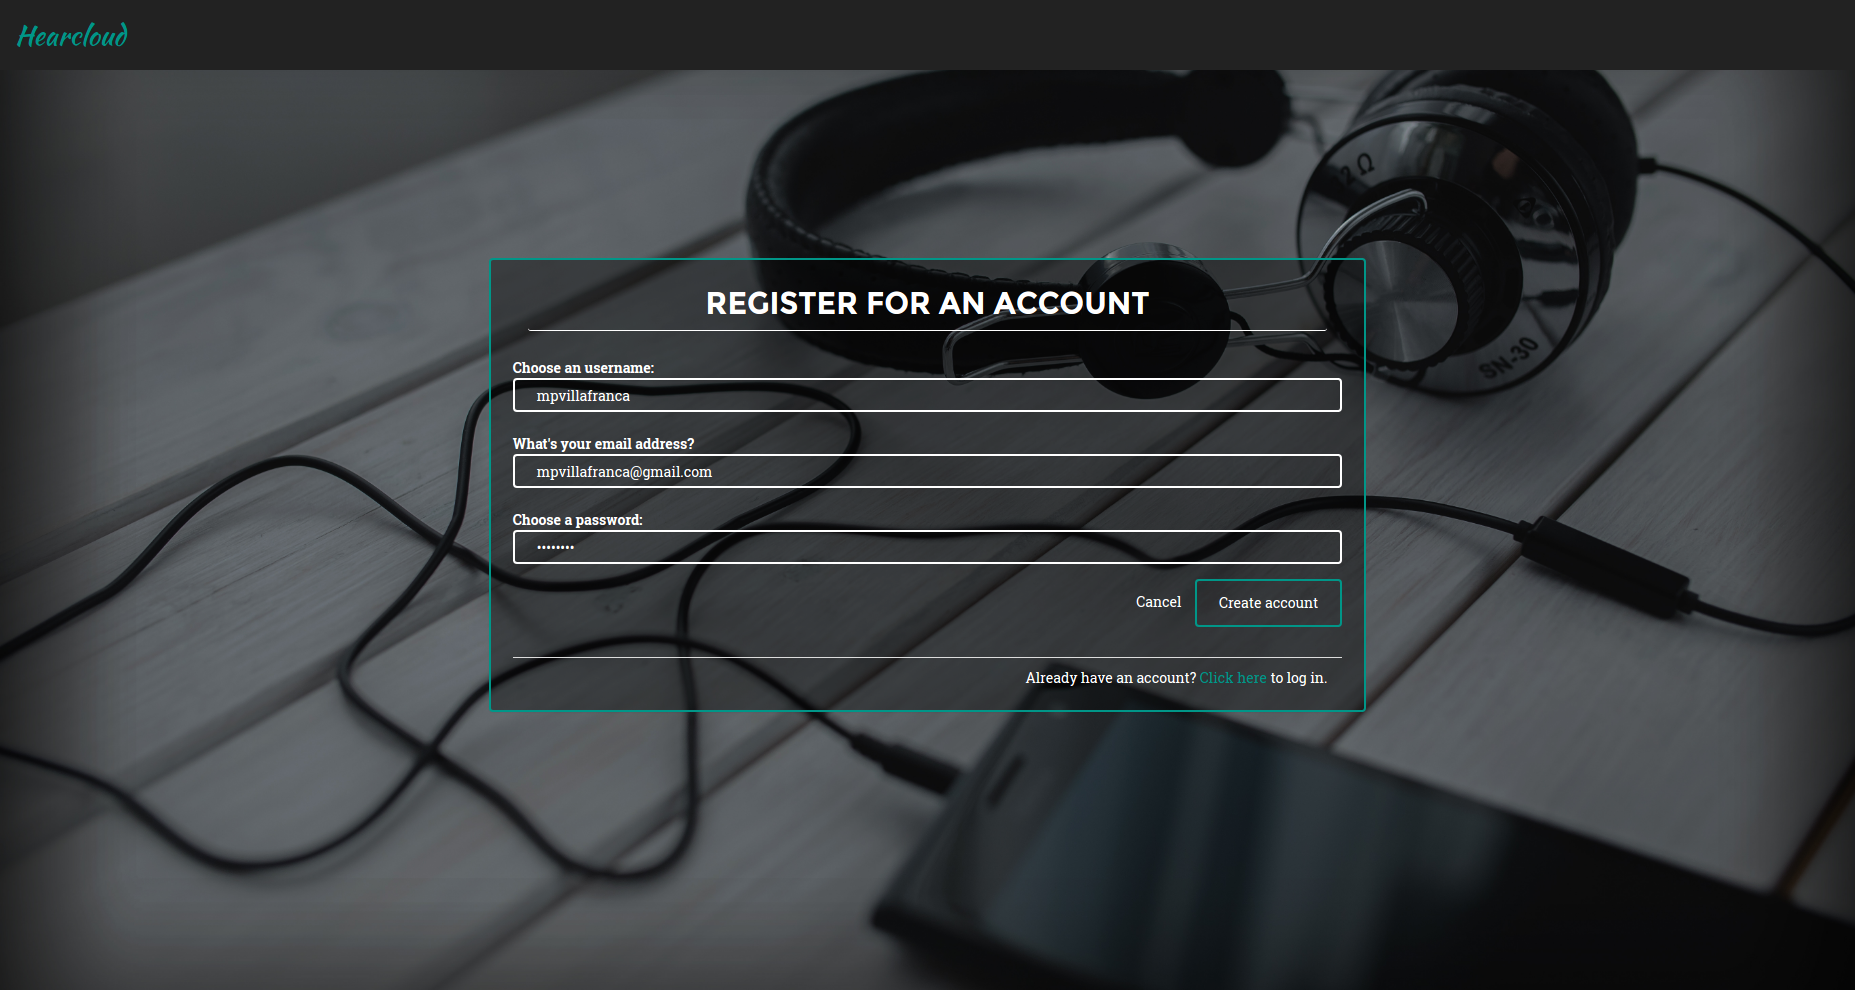
\includegraphics[scale=0.2]{../images/um/um_2.png}
\caption{Página de registro de usuarios}
\end{figure}

Al igual que en el caso anterior, la página de inicio de sesión, en la que se muestra un formulario para introducir nombre de usuario y contraseña, da la posibilidad de cancelar el inicio o de acceder al formulario de registro.

\begin{figure}[H] 
\centering 
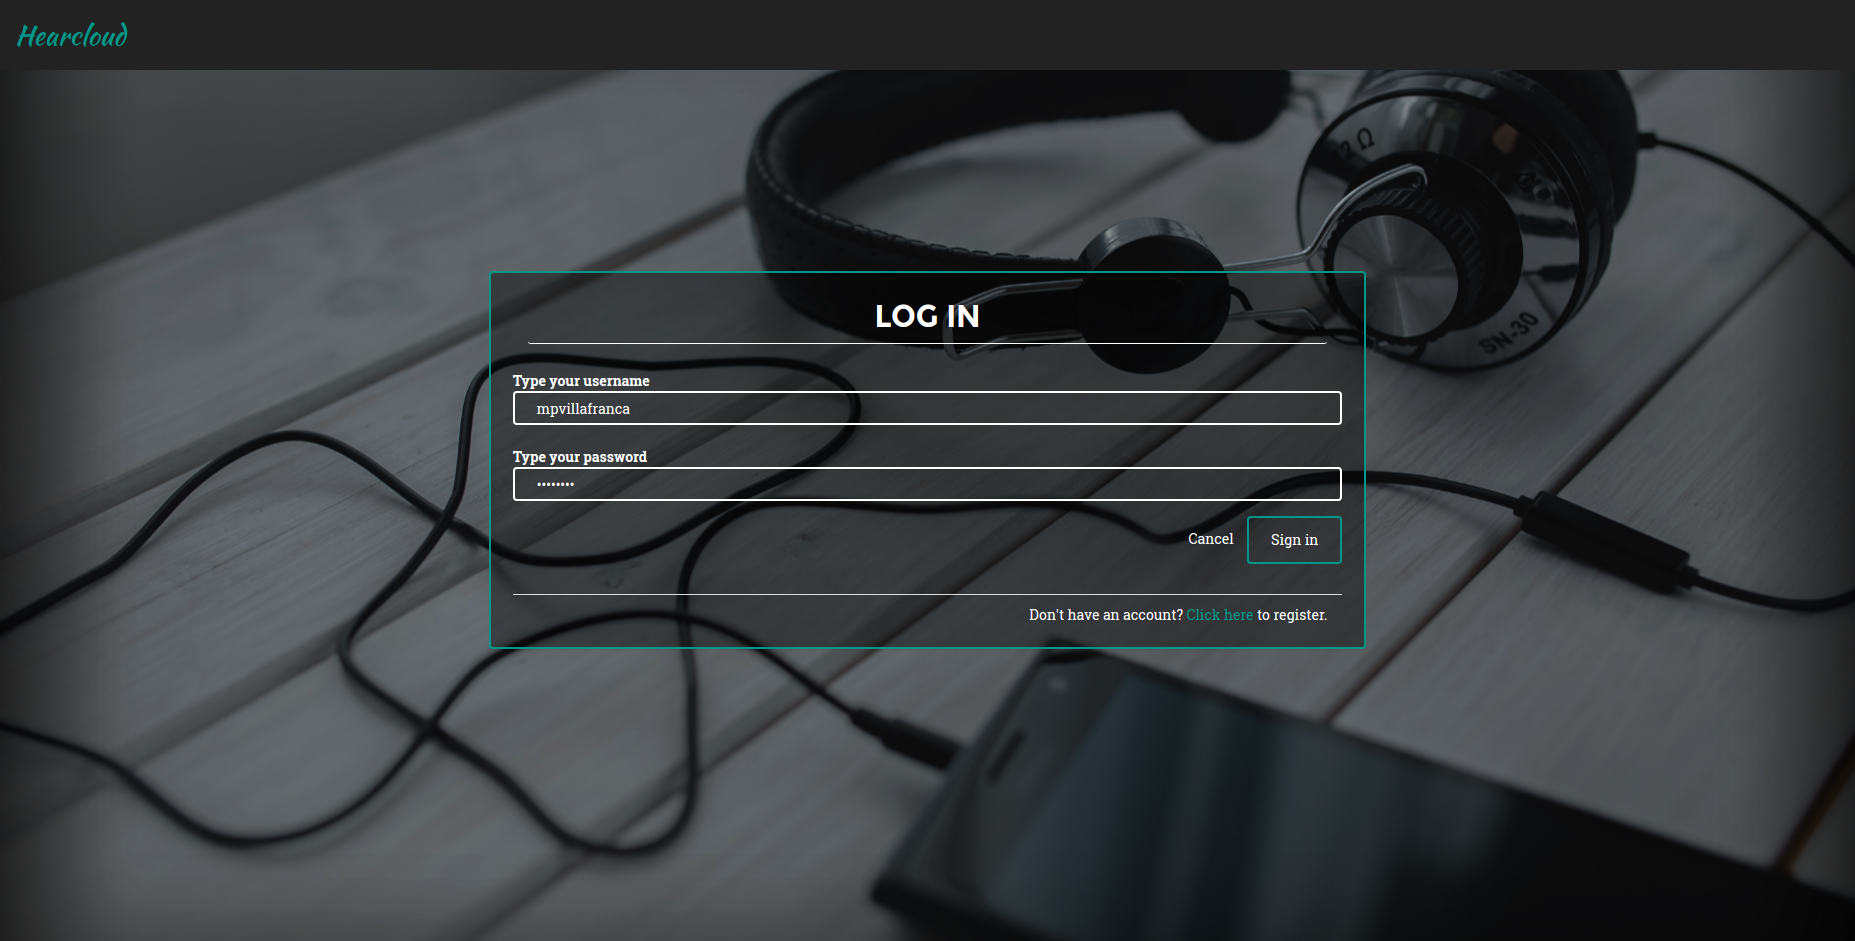
\includegraphics[scale=0.2]{../images/um/um_3.png}
\caption{Página de inicio de sesión de usuarios}
\end{figure}

\subsection{Panel principal del sistema: Canciones}

Es la vista principal del sistema para los usuarios que han iniciado sesión en la plataforma. Si es la primera vez que acceden, el panel central se mostrará vacío. Las canciones que el usuario vaya subiendo irán apareciendo en dicho panel, donde se muestra información básica acerca de la canción (imagen, título, artista, album, duración y fechas de subida y modificación). Por cada canción, aparecen tres acciones posibles a realizar en forma de botones: reproducir, descargar y eliminar.

Si se hace click en el botón de reproducir, se abrirá el reproductor integrado dentro del sistema, donde se muestran título y artista de la canción, junto a su portada y forma de onda. Además, nos podremos desplazar a lo largo de la canción para adelantarla o atrasarla. Se proporciona, por último, un boton que permite pausar la reproducción y reanudarla de nuevo en el punto en que se quedó.

Por otra parte, se ofrece la posibilidad al usuario de descargar el fichero de audio de vuelta a su sistema local, dándole la opción de realizar una conversión a otro formato de audio. Si la canción ha sido subida en un formato sin compresión (wav o aiff), las opciones de descarga serán cualquiera de los cuatro formatos disponibles (wav, aiff, m4a y mp3). Si la canción se subió en un formato con compresión (m4a y mp3), solo se podrán realizar conversiones entre dichos formatos.

\begin{figure}[H] 
\centering 
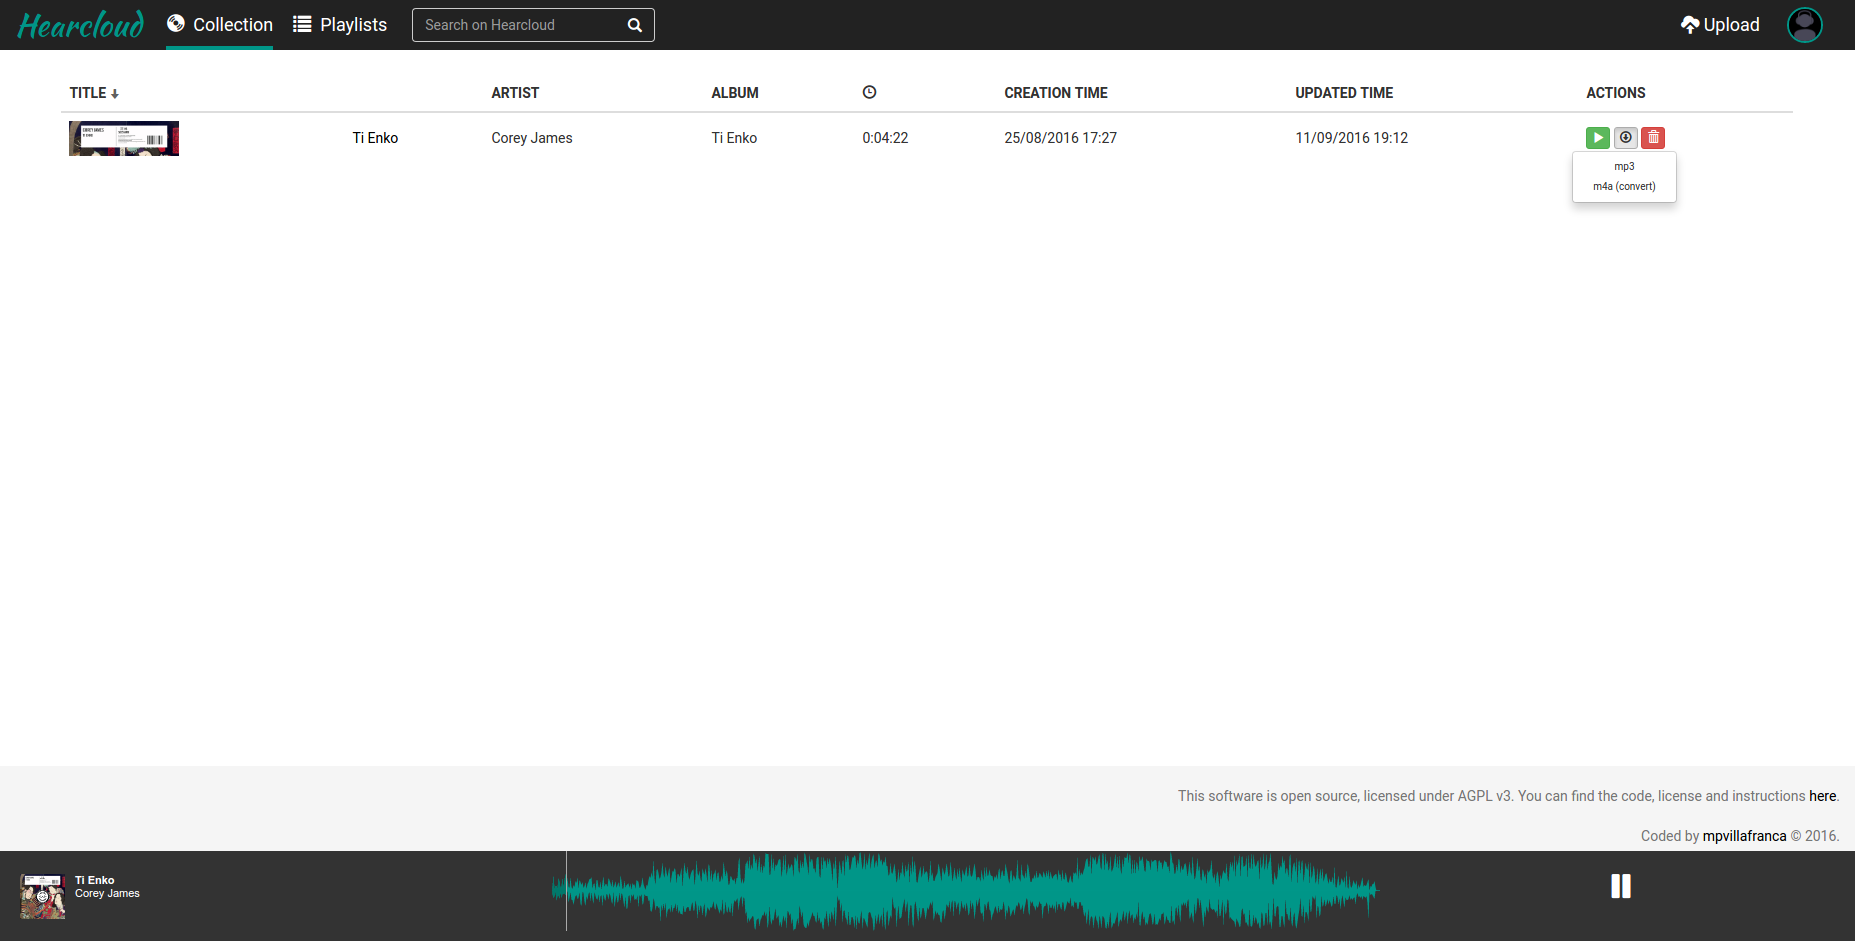
\includegraphics[scale=0.2]{../images/um/um_4.png}
\caption{Página principal (usuario autenticado)}
\end{figure}

Además, el usuario puede acceder a los detalles de la canción haciendo click en ella. En esta nueva ventana, se muestran todos los metadatos de la canción y se ofrece la posibilidad de editarlos mediante el correspondiente botón. Además, se vuelven a mostrar las opciones de reproducción, descarga y eliminación anteriores, cuyo comportamiento es idéntico al descrito anteriormente.

\begin{figure}[H] 
\centering 
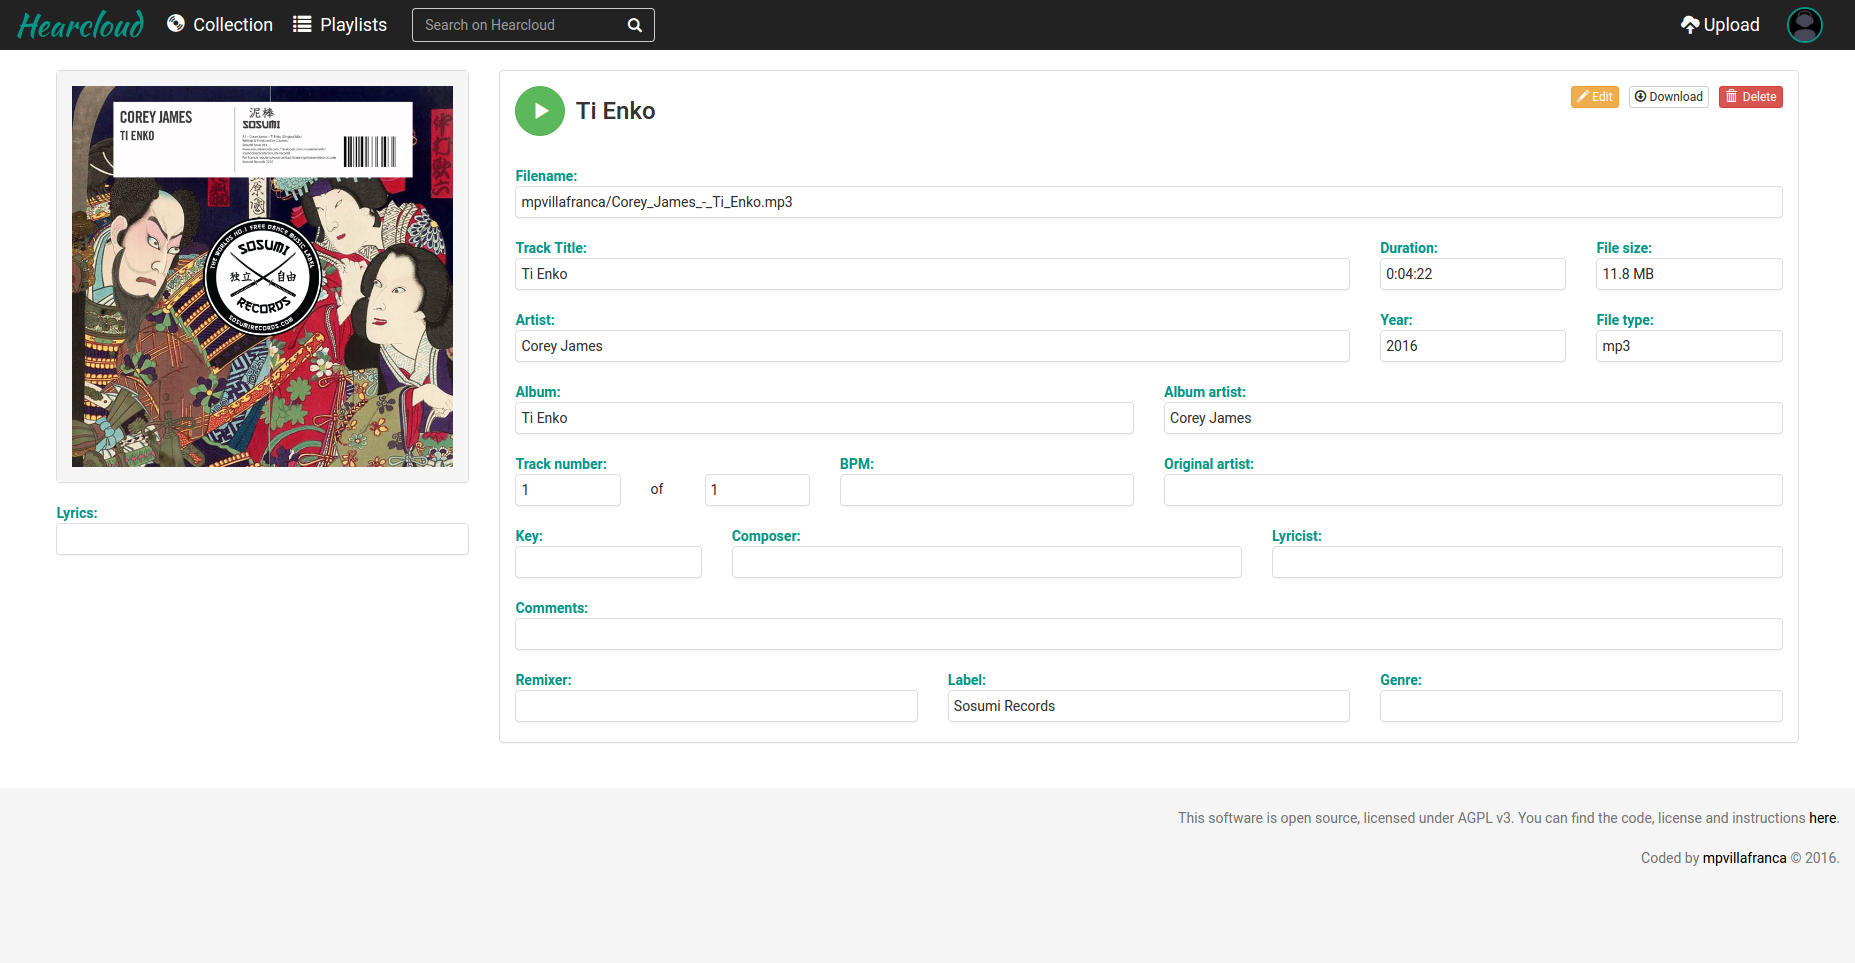
\includegraphics[scale=0.2]{../images/um/um_5.png}
\caption{Página del detalle de una canción}
\end{figure}

\subsection{Subida de ficheros}

Esta página es accesible mediante el botón \textit{Upload} situado en la barra de navegación del sistema. En ella, se da la posibilidad al usuario de subir a la plataforma cuantas canciones desee en una sola vez, aunque también puede seleccionar subir únicamente determinadas canciones de todas las seleccionadas inicialmente. Además, se ha implementado una \textit{drop zone}, donde el usuario puede arrastrar las canciones directamente desde el sistema sin necesidad de pulsar sobre el botón \texttt{Add files}.

\begin{figure}[H] 
\centering 
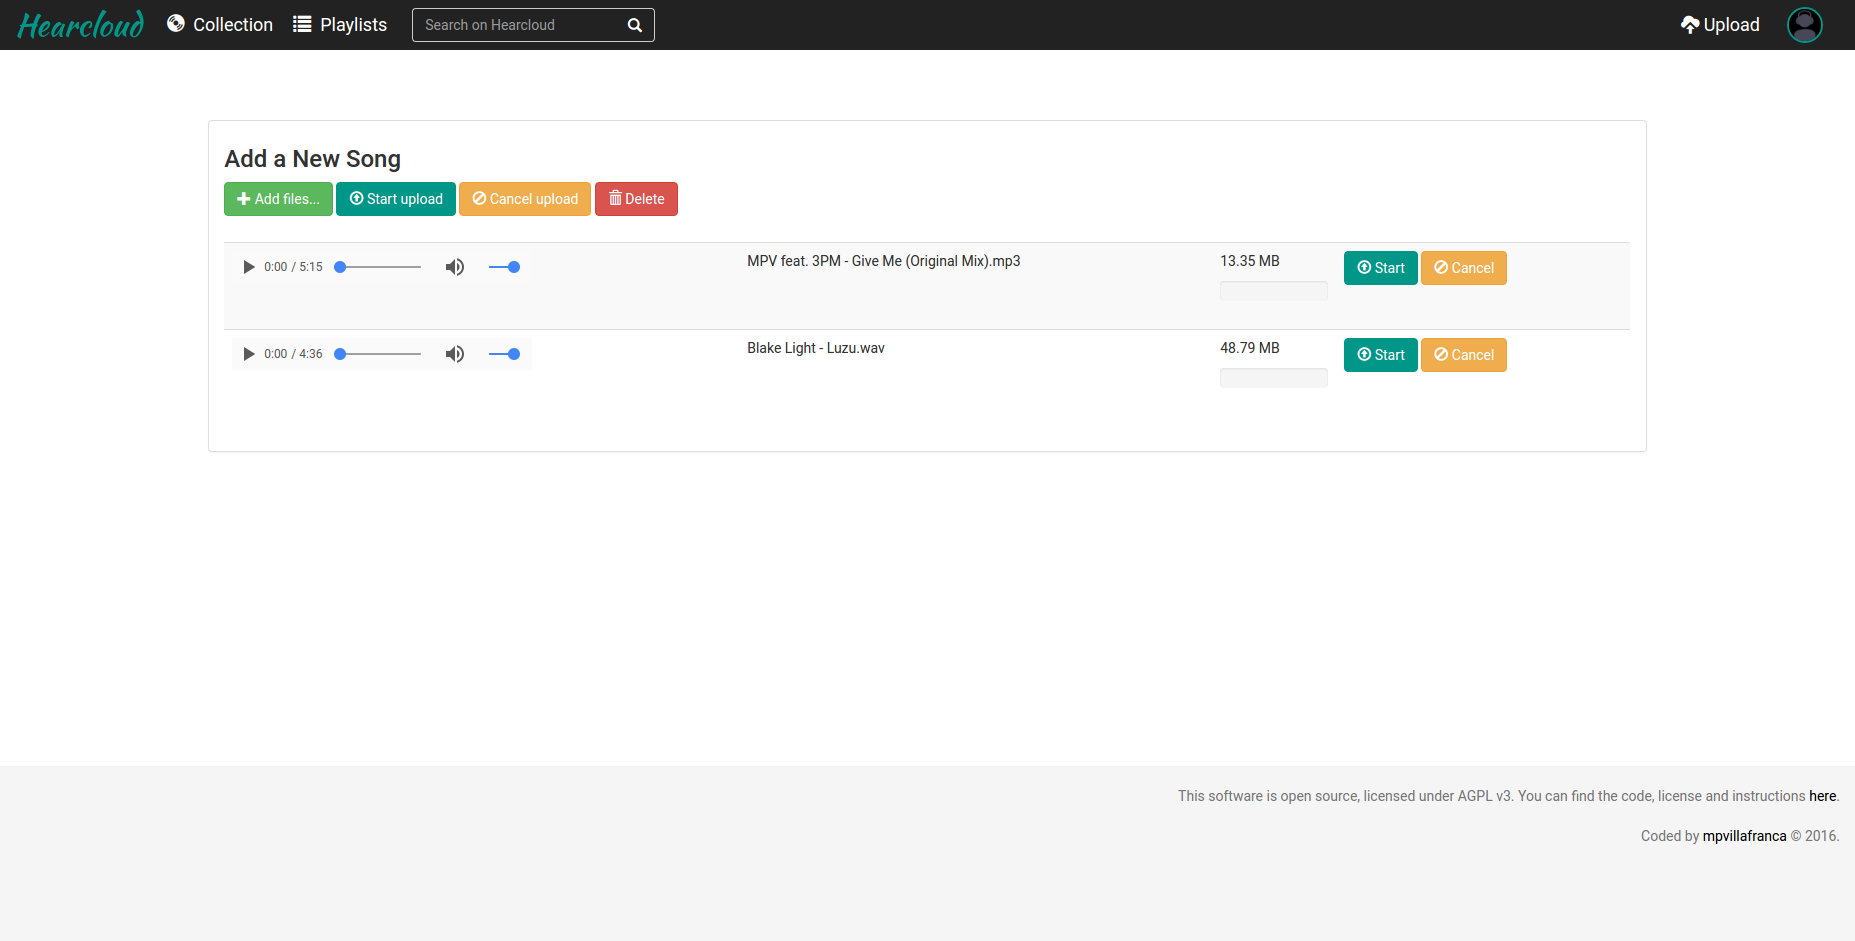
\includegraphics[scale=0.2]{../images/um/um_6.png}
\caption{Página de subida de canciones}
\end{figure}

\subsection{Panel perfil de usuario}

Este panel es accesible a través de la imagen de perfil del usuario situada en el borde superior derecho de la barra de navegación. En ella, se muestra la imagen de perfil del usuario, sus datos básicos y un contador sobre el número de canciones y listas de reproducción que tiene en su sistema.

\begin{figure}[H] 
\centering 
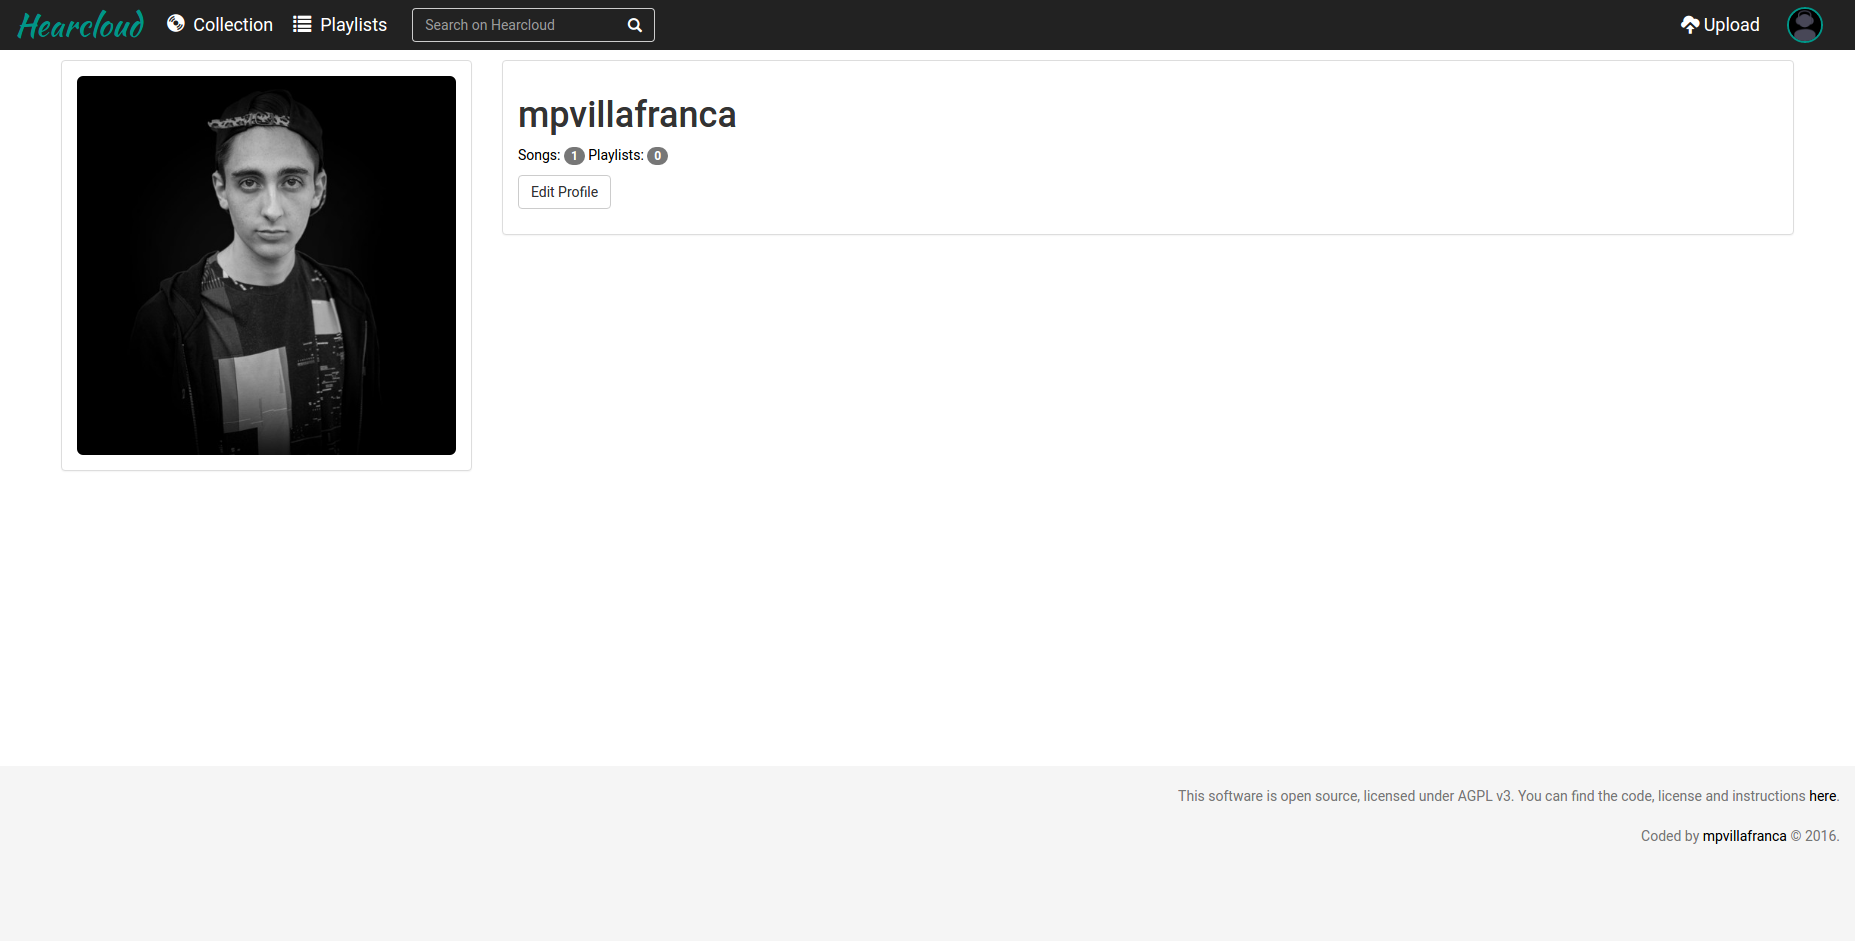
\includegraphics[scale=0.2]{../images/um/um_7.png}
\caption{Página del perfil de usuario}
\end{figure}

\subsection{Panel de administración}

Django ofrece un panel de administración accesible a través de la url \texttt{/admin}, al que podrán acceder todos los usuarios que tengan activado el atributo \texttt{is\_staff}. Las opciones que aquí se les muestren dependerán de los permisos que se les concedan. 

\begin{figure}[H] 
\centering 
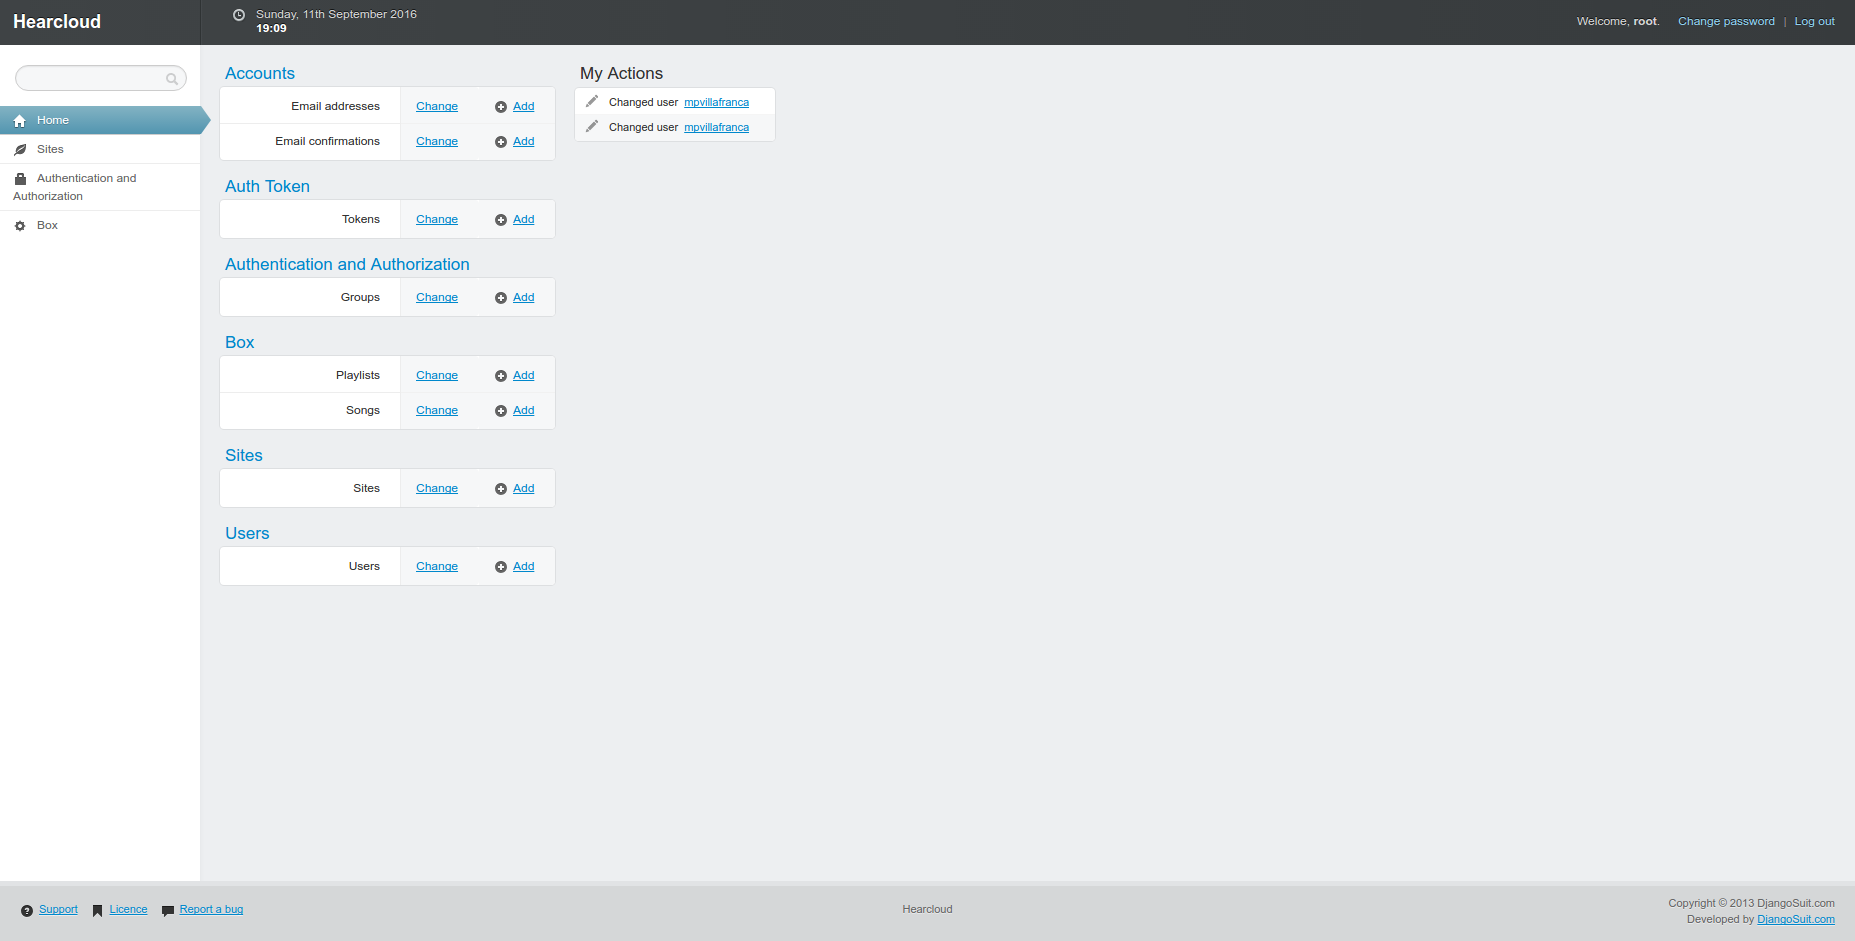
\includegraphics[scale=0.2]{../images/um/um_8.png}
\caption{Panel de administración de Django. Vista principal.}
\end{figure}

Si el usuario que accede posee todos los permisos o es superusuario, se desplegarán todas las opciones disponibles. Con él, podremos gestionar los usuarios y grupos del sistema y los ficheros y listas de reproducción que éstos almacenen.

\begin{figure}[H] 
\centering 
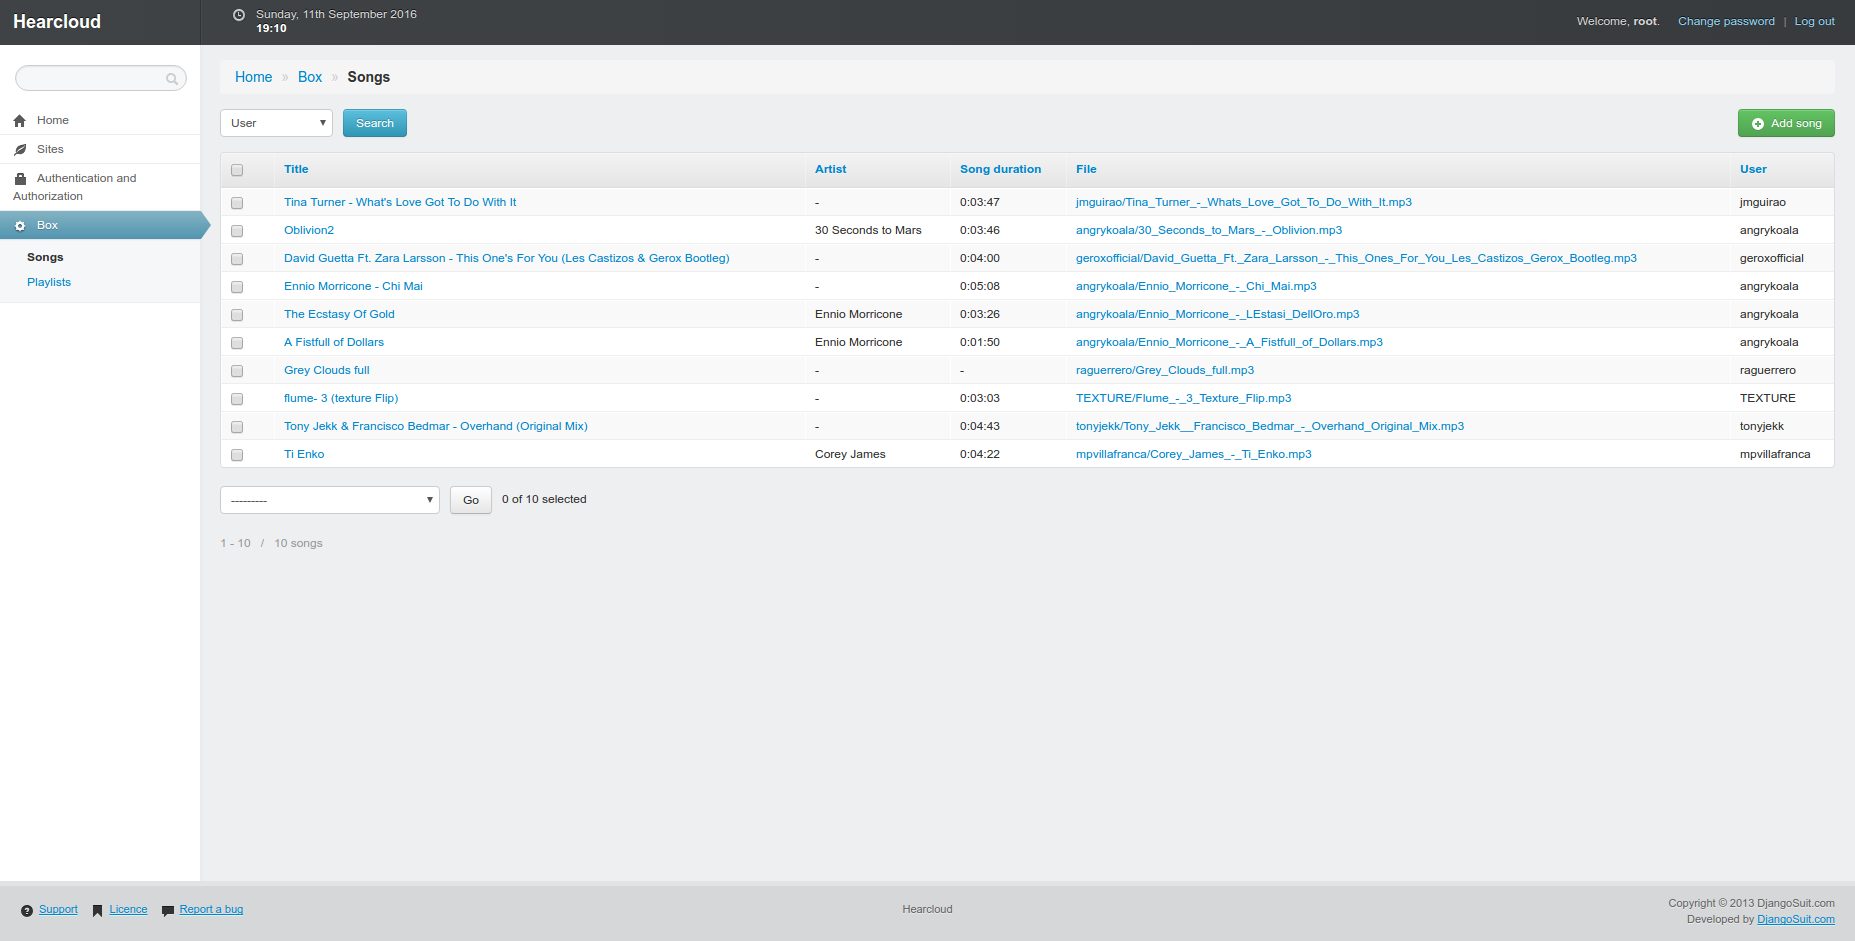
\includegraphics[scale=0.2]{../images/um/um_9.png}
\caption{Panel de administración de Django. Lista de canciones del sistema.}
\end{figure}

\subsection{Diseño adaptativo. Versión móvil}

Durante el desarrollo del sistema se ha tenido en cuenta que la plataforma se adapte lo máximo posible a los diferentes dispositivos desde los que se pueda acceder a ella, por lo que todas las secciones descritas anteriormente, deberían de visualizarse correctamente sin importar desde dónde se esté accediendo.

\begin{figure}[H]
\minipage{0.32\textwidth}
  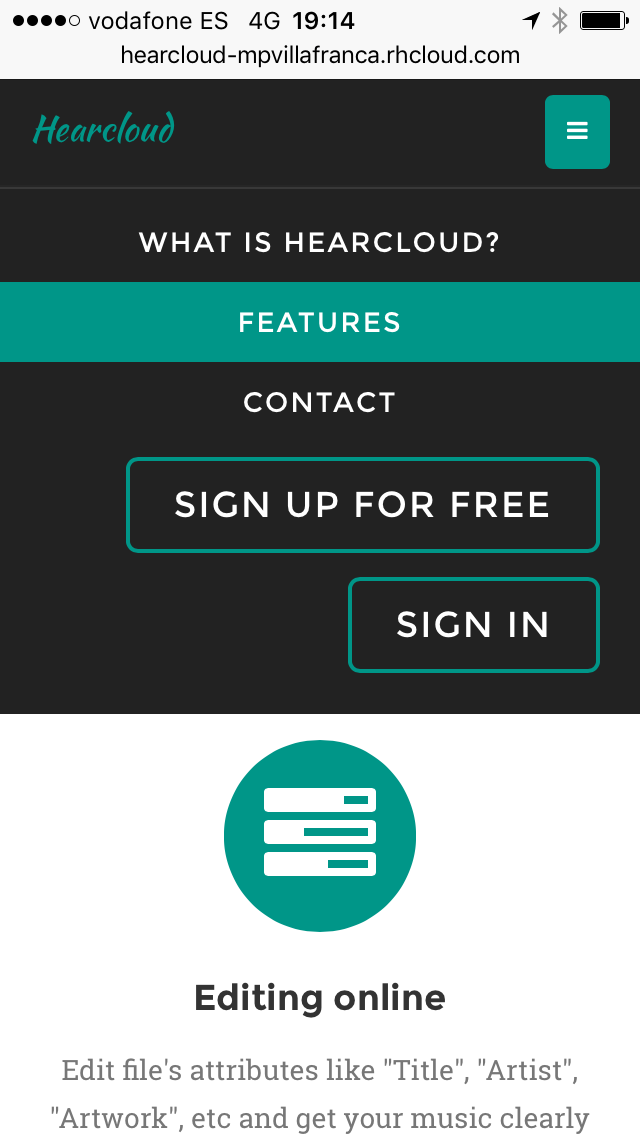
\includegraphics[width=\linewidth]{../images/um/um_10.png}
  \caption{Página principal (usuario no autenticado) en iPhone 6S}
\endminipage\hfill
\minipage{0.32\textwidth}
  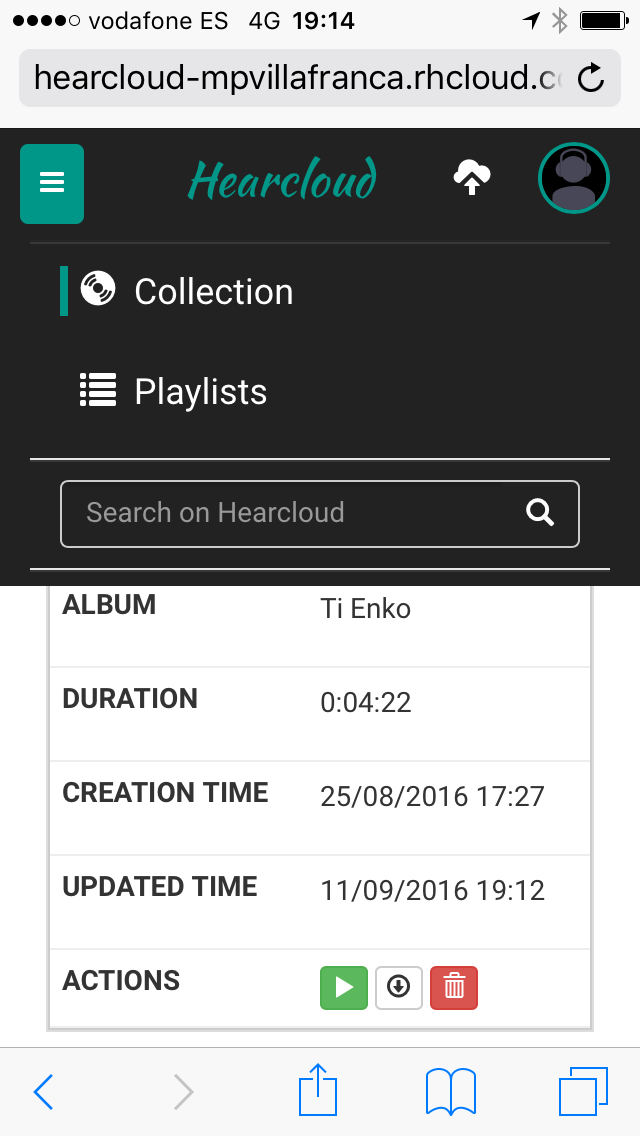
\includegraphics[width=\linewidth]{../images/um/um_11.png}
  \caption{Página principal (usuario autenticado) en iPhone 6S}
\endminipage\hfill
\end{figure}

\newpage

\newpage

\begin{thebibliography}{99}
	\addcontentsline{toc}{chapter}{Bibliografía}
\label{cap:bibliografia}

% ********************************************************************
% Bibliografía general
% ********************************************************************
\subsubsection*{Articulos y referencias generales consultados durante el desarrollo proyecto:}

% Comparación de tags entre diferentes formatos
\bibitem{TMMT} Tag Mapping - Mapping Tables \url{http://wiki.hydrogenaud.io/index.php?title=Tag_Mapping}

% Audio file metadata
\bibitem{PUMID3H} Python Useful Modules. ID3 Handling \url{https://wiki.python.org/moin/UsefulModules#ID3_Handling}

% Formularios con Ajax
\bibitem{DaAFS} Django and AJAX Form Submissions - Say ``Goodbye'' to the Page Refresh \url{https://realpython.com/blog/python/django-and-ajax-form-submissions/}


A continuación se presenta la bibliografía consultada en cada uno de los apartados de este proyecto.

\bigskip

% ********************************************************************
% Introducción
% ********************************************************************
\subsubsection*{Introducción.}

\bibitem{HDRDS} Historia del registro del sonido. \url{https://es.wikipedia.org/wiki/Historia_del_registro_del_sonido}

% ********************************************************************
% Objetivos
% ********************************************************************
\subsubsection*{Objetivos.}

% ********************************************************************
% Planificación y Analisis
% ********************************************************************
\subsubsection*{Planificación y análisis.}

\bibitem{Spotify} Spotify. \url{https://www.spotify.com/}

\bibitem{WikiSpotify} Wikipedia: Spotify. \url{https://en.wikipedia.org/wiki/Spotify}

\bibitem{SCYUYOM} Spotify: Can you upload your own music? \url{https://community.spotify.com/t5/Desktop-Linux-Windows-Web-Player/Can-you-upload-your-own-music/m-p/41511}

\bibitem{VLPPPSP} Spotify: ¿Vale la pena pagar por spotify premium? \url{http://curiotek.com/2015/03/01/vale-la-pena-pagar-por-spotify-premium/}

\bibitem{Soundcloud} Soundcloud. \url{https://soundcloud.com}

\bibitem{WikiSoundcloud} Wikipedia: Soundcloud. \url{https://en.wikipedia.org/wiki/SoundCloud}

\bibitem{ACP} Amazon Cloud Player. \url{https://music.amazon.com}

\bibitem{AUMIYML} Amazon Music. Help \& Customer Service. \url{https://www.amazon.com/gp/help/customer/display.html/ref=hp_bc_nav?ie=UTF8&nodeId=201377280}

\bibitem{GPM} Google Play Music. \url{https://www.play.google.com/music}

\bibitem{WikiGPM} Wikipedia: Google Play Music. \url{https://es.wikipedia.org/wiki/Google_Play_Music}

\bibitem{MMC} My Music Cloud. \url{https://www.mymusiccloud.com}

\bibitem{FAQMMC} My Music Cloud. Preguntas frecuentes. \url{http://support.mymusiccloud.com/}

\bibitem{GMELNEL} ``Guardar música en la nube es legal''. Laia Reventós, 24/08/2011. \url{http://elpais.com/diario/2011/08/24/radiotv/1314136802_850215.html}

% ********************************************************************
% Diseño
% ********************************************************************
\subsubsection*{Diseño.}

% ********************************************************************
% Implementación
% ********************************************************************
\subsubsection*{Implementación.}

% ********************************************************************
% Pruebas
% ********************************************************************
\subsubsection*{Pruebas.}

% ********************************************************************
% Pruebas
% ********************************************************************
\subsubsection*{Conclusiones.}

% ********************************************************************
% APIs
% ********************************************************************
\subsubsection*{Páginas de consulta sobre licencias y APIs del software utilizado:}
\bibitem{CC} Creative Commons. \url{http://creativecommons.org/licenses/}
\bibitem{Dj} Django. \url{https://www.djangoproject.com/}
\bibitem{J2} Jinja2. \url{https://www.djangoproject.com/}

\bibitem{TCI} {\tt Travis CI}. \url{http://docs.travis-ci.com/}

\bigskip


% ********************************************************************
% Otro material
% ********************************************************************
\subsubsection*{Otro material}
\begin{itemize}
	\item Diversas consultas puntuales al sitio {\tt Stack OverFlow}.
	\item Material docente de las asignaturas \textbf{Fundamentos de Ingeniería del Software}, \textbf{Desarrollo de Aplicaciones para Internet} e \textbf{Infraestructura Virtual} impartidas en el \textbf{Grado en Ingeniería Informática} en la \textbf{Universidad de Granada}.
\end{itemize}

\end{thebibliography}


\thispagestyle{empty}
\end{document}
